\pagebreak
\section{Gegenmaßnahmen}
Wie in Abschnitt \ref{sec:explainersub} bereits aufgeführt,
gehören zu einem Buffer-Overflow-Angriff mehrere kombinierte Teile. Wenn
man nun verhindern möchte, dass ein Programm über diesen Angriff gestürzt werden
kann, so hat man mehrere Möglichkeiten diese Teile aufzuhalten oder die Kombination
zu blockieren. Es folgen mehrere Möglichkeiten, grob nach Aufwand (für den Entwickler) sortiert.
\subsection{Übersicht der Maßnahmen}
Low-Level:
    \begin{itemize}
        \item Hardware-basierte Lösungen
        \item Betriebssystembasierte Ansätze
    \end{itemize}
Passive Härtung der Programme:
    \begin{itemize}
        \item C Range Error Detector und Out Of Bounds Object
        \item Safe Pointer Instrumentalisierung
        \item Manuelles Buffer-Overflow Blocken (Input-Bereinigung)
    \end{itemize}
Aktive (Analysierende) Lösungen:
    \begin{itemize}
        \item Statische Code-Analyse
        \item Stack-Schutz mit ``Canary'' (Zufallszahl)
    \end{itemize}


\subsection{Low-Level Probleme}
Sowohl Hardwarelösungen als auch Betriebssystembasierte Lösungen haben
das grundlegende Problem, dass die Verhinderung von Buffer-Overflows zu
ungewünschten Nebeneffekten führen kann. Es ist auf jeden Fall möglich,
jegliche Overflows zu verhindern - dabei werden jedoch auch vom
Entwickler gewünschte Overflows verhindert, sodass Programme nicht mehr
ordentlich funktionieren. Manchmal wird aus gründen der Effizienz ein
Buffer zum Überlaufen gebracht, ohne dass dieser Überlauf unkontrolliert
ist. Leider ist es Praktisch nicht umsetzbar, in einer Hardwarelösung
zu entscheiden, welcher Buffer-Overflow böswillig ist.



\subsection{Out Of Bounds Object}
Ein Out Of Bounds Object ist eine Vereinfachte Lösung um Referenzen ungefährlich zu machen.
Es wird verhindert, dass auf Speicher außerhalb des Programms zugegriffen wird, indem Jede
Adresse welche nicht im spezifizierten Bereich liegt auf ein bestimmtes Objekt, das sogenannte
"Out Of Bounds Object" verweist. Dadurch kann innerhalb des laufenden Programms erkannt werden, das
etwas falsch gelaufen ist. Diese Methode ist nicht gängig, da sie technisch gesehen
umgangen werden kann, solange der Angreifer weiß, welcher Speicherbereich für das Programm
vorgesehen ist.

\subsection{Statische Analyse}
Wenn das Programm bereits vor der Ausführung analysiert wird, kann ein
Tool bestimmen, an welchen stellen Schwachstellen vorhanden sind und
ggf. vorschlagen, wie diese behoben werden können. Leider ist bei größeren
Projekten die Aussage, dass keine Schwachstellen mehr vorhanden seien
unmöglich zu treffen.

\subsection{Canaries}
Die Bezeichnung Canary (Engl. Kanarienvogel) stammt aus der Verwendung der Kanarienvögel als
Indikator für Gas in Mienen. Die Canaries im Code werden als Stack-Schutz verwendet. Das bedeutet,
dass beispielsweise Zufallszahlen im Programm auf dem Stack sind und bei einem Buffer-Overflow-Angriff
überschrieben werden. Ein Tool wie StackGuard kann dann anhand der Änderung einen Fehler feststellen und
die Ausführung des Programms abbrechen.

%TODO: ASLR Beschreiben

\subsection{Code-Beispiel}
    \begin{center}
        %TODO: Besseres Beispiel finden.
        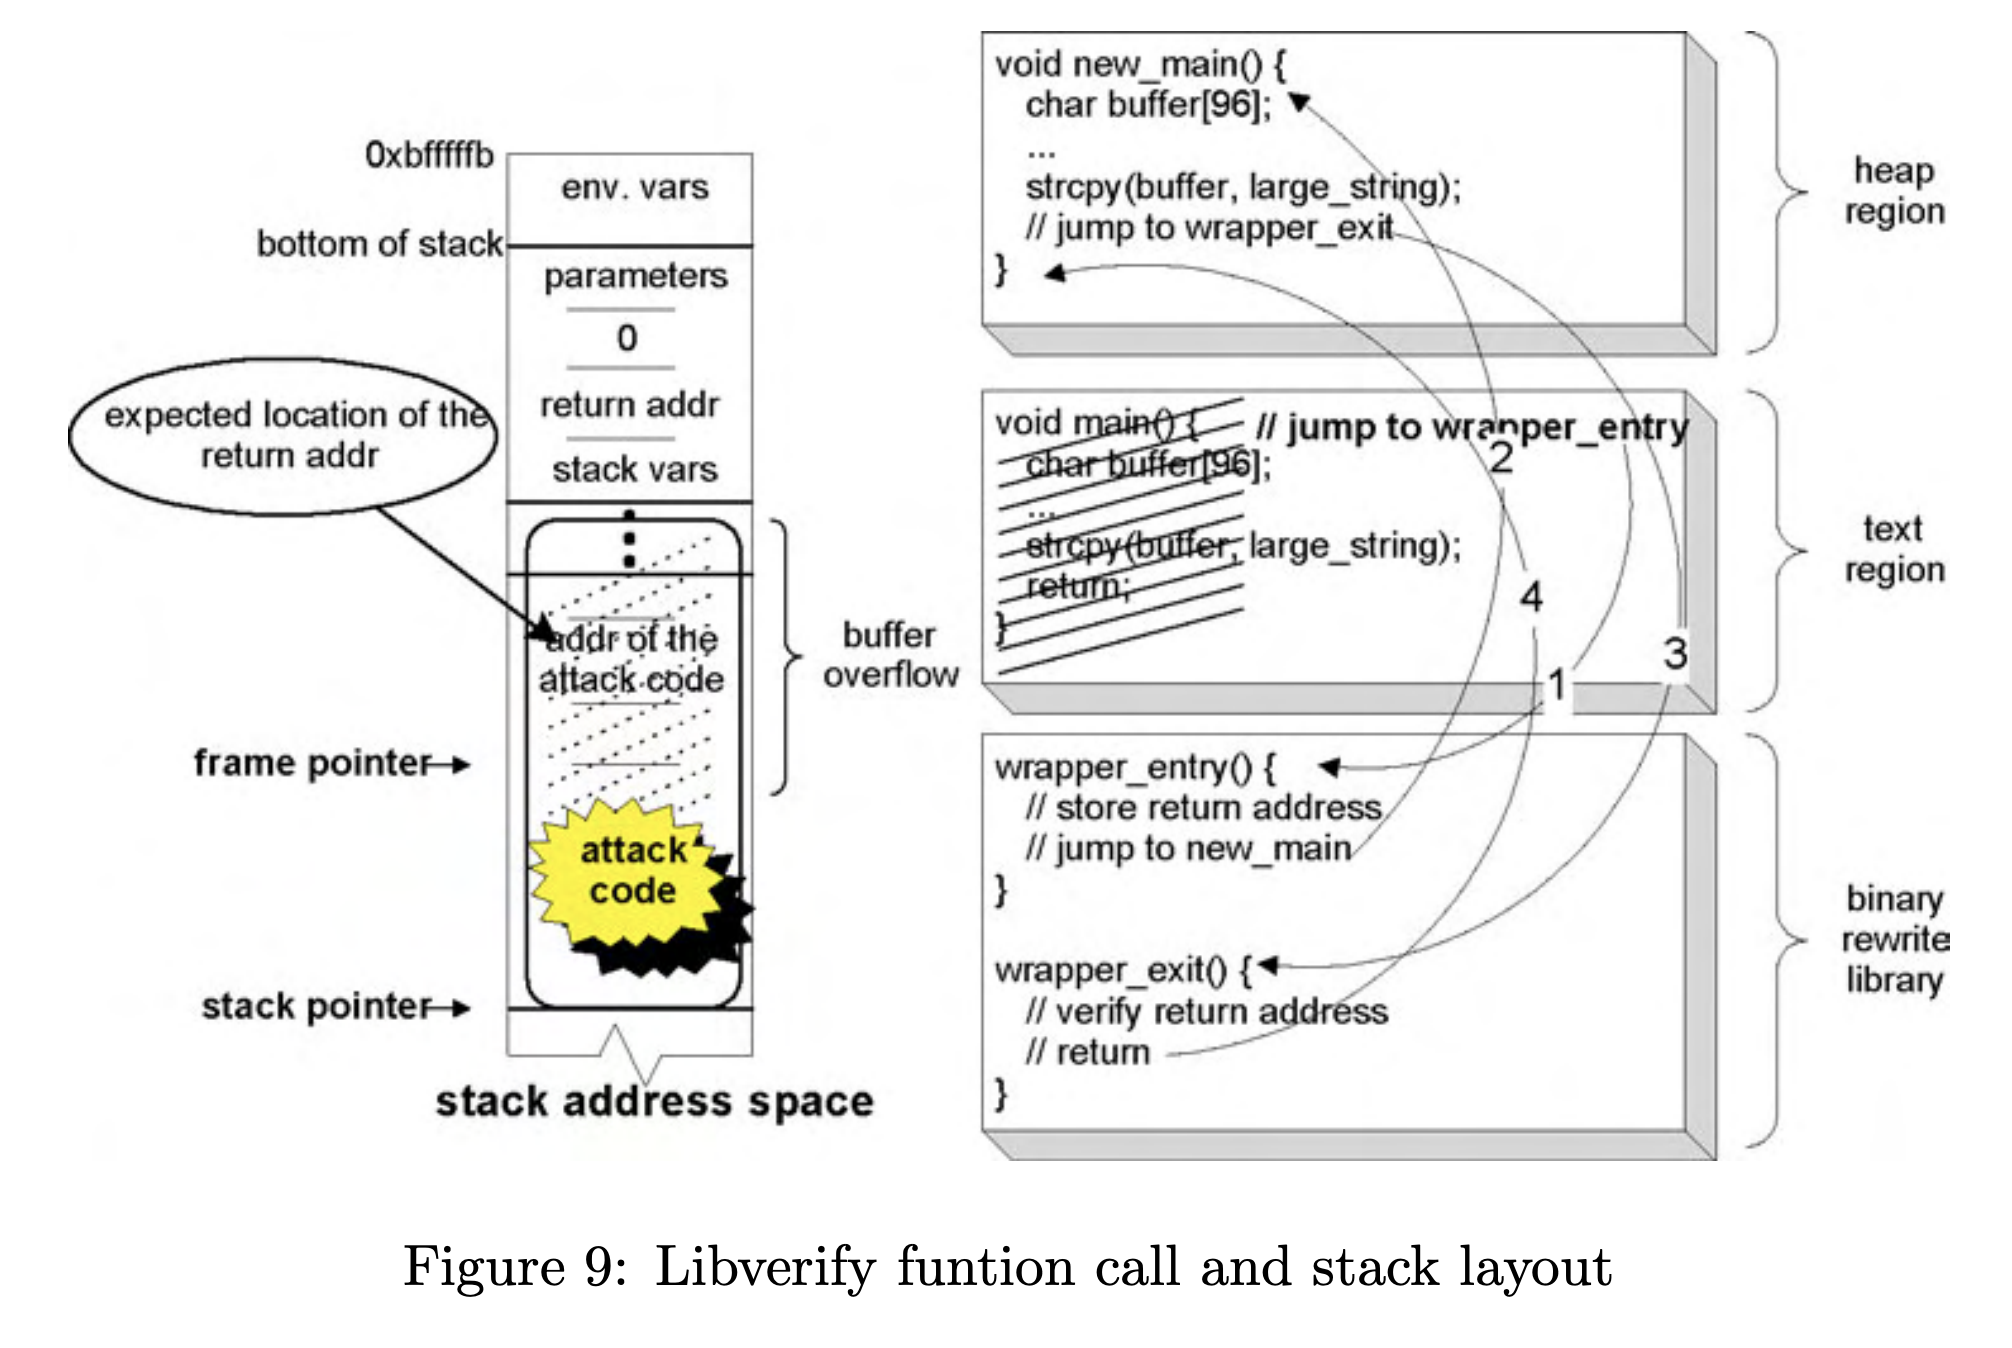
\includegraphics[width=\textwidth,height=0.75\textheight,keepaspectratio]{images/Libverify.png}
    \end{center}

\subsection{Testen}
Es gibt mehrere Möglichkeiten um kompilierte Programme auf ihre Sicherheit
und Robustheit zu testen. Diese beiden Qualitätsmerkmale sind vor Allem
im Bezug zu Buffer-Overflows am wichtigsten. Wartbarkeit und Erweiterbarkeit
sind langfristig auch zu beachten, da es bei Änderungen am Quellcode
zu Fehlern kommen kann, welche Schwachstellen herbeibringen.
Mit Werkzeugen wie Sonar lint können vor allem häufig auftretende Fehler entdeckt
werden.
Im Bereich der Overflow Payloads gibt es mehrere Werkzeuge um Fuzzy Testing
zu betreiben. Beim Fuzzy Test wird strukturiert zufällig auf eine 
potentielle Schwachstelle getestet, wobei die tatsächlichen aufrufe
von einem sogenannten Fuzzer erstellt werden.
Als Alternative zum Fuzzing gibt es Spezifische Payloads und
Escape-Sequenzen welche - auch automatisiert - getestet werden können.

